
\section{Nattino et al. (2020)}


% -------------------------------------------------------------------------

\begin{frame}
  \frametitle{Nattino et al. (2020)}
  
  \textbf{Goal:} Compare effectiveness of trauma centers as measured
  by \emph{emergency department mortality}, for three classes of
  trauma center, 
  \begin{itemize}
  \item level 1 trauma center (TC I) \medskip 
  \item level 2 trauma center (TC II) \medskip 
  \item nontrauma center (NTC) \medskip 
  \end{itemize}

  Counterfactual of interest: \footnotesize\textit{``\ldots the key
    research question is whether TC II is a justified investment of
    limited trauma care resources. If trauma patients treated at TC II
    had, instead, been treated at TC I or NTC, would their outcomes
    have been different?''} -- p. 1 \normalsize
  
\end{frame}

% -------------------------------------------------------------------------

\begin{frame}
  \frametitle{Assumptions}

  Let $Y_\ell^{(z)}$ for $z \in \{1,2,3\}$ denote the counterfactual
  outcome (1 for death, 0 for survival) for unit $\ell=1,\ldots, N$.

  \medskip

  The observed value is
  $Y_\ell = Y^{\text{obs}}_\ell = \sum_{z=1}^{3} I(Z_\ell = z)
  Y_\ell^{(z)}$

  \medskip

  $\mathbf{X}_\ell$ is a vector of pre-treatment covariates  \medskip 

  \begin{enumerate}[1. ]
  \item SUTVA: no interference between units, no multiple versions of
    same treatment
  \item Positivity
    \begin{align*}
      0 < \Pr(Z_\ell = z \mid Y_\ell^{(1)}, Y_\ell^{(2)},
      Y_\ell^{(3)}, \mathbf{X}_\ell) < 1 \quad \forall z \in \{1,2,3\}
    \end{align*}
    \item
  Strong ignorability
  \begin{align*}
    Z_\ell \ind Y_\ell^{(1)}, Y_\ell^{(2)},
      Y_\ell^{(3)} \mid \mathbf{X}_\ell
  \end{align*}
  \end{enumerate}

\end{frame}

% -------------------------------------------------------------------------

\begin{frame}
  \frametitle{Three-way matching}
  
  \textbf{Idea}: replicate conventional block randomization design,
  using triplets of units containing all treatment assigments
  $z=1,2,3$ \medskip 

  Let $\mathcal{I}$, $\mathcal{J}$, and $\mathcal{K}$ denote the sets
  of indices of subjects in subject.  We will create
  $S = \min\{n_1, n_2, n_3\}$ matched triplets.  Will match on
  variables $\mathbf{V}$ (either covariates $\mathbf{X}$ or the GPS).
  \medskip

  \begin{itemize}
  \item Define a distance metric $d^3(i,j,k)$, $i \in \mathcal{I},
    j \in \mathcal{J}, k\in\mathcal{K} $ as a function of
    $\mathbf{V}_i$, $\mathbf{V}_j$ and $\mathbf{V}_k$, with additivity property
    \begin{align*}
      d^3(i,j,k) = d^2(i,j) + d^2(i,k) + d^2(j,k)
    \end{align*}
  \item Denote set of possible matches as
    $\mathcal{M} = \{i, j_i, k_i\}_{i \in \mathcal{I}}$, where the
    units $j_i$ and $k_i$ are matched to units $i$ \medskip 
  \item Goal is to find $\mathcal{M}$ to minimize
    $D(\mathcal{M}) = \sum_{i\in\mathcal{I}}^{}d^3(i,j_i,k_i)$
  \end{itemize}



\end{frame}

% -------------------------------------------------------------------------




\begin{frame}
  \frametitle{Triplet matching algorithm}
  
  Rough outline: \medskip

  
  \begin{enumerate}[(i)]
  \item Select two treatment groups arbitrarily, and optimally match
    them into pairs \medskip 
  \item Optimally match units in the third treatment group to each of
    the pairs from step \textcolor{burntorange}{(i)} (keeping previous
    pairs fixed) \medskip 
  \item Switch the two fixed treatment groups, and then optimally
    match units from the third treatment group \medskip
  \item Iterate through step \textcolor{burntorange}{(iii)} until
    total distance cannot be decreased further
  \end{enumerate}

  \medskip 

  This method produces sets of matched triplets, but each step only
  requires two-way matching

  
\end{frame}

% -------------------------------------------------------------------------

\begin{frame}
  \frametitle{Inference on mortality differences}
  
  Denote treatment and outcome vectors for triplet $s=1,\ldots,S$ as
  $\mathbf{Z}_s = \{Z_{s1}, Z_{s2}, Z_{s3}\}$ and
  $\mathbf{Y}_s = \{Y_{s1}, Y_{s2}, Y_{s3}\}$

  \medskip 

  \begin{itemize}
  \item Fisher's sharp null hypothesis of no effect at all:
    $H_0 = Y^{(1)}_{sr} = Y^{(2)}_{sr} = Y^{(3)}_{sr}$ for subject
    $r=1,2,3$. \medskip 
  \item Consider two comparisons: \smallskip
    \begin{enumerate}[(1)]
    \item NTC vs TC overall ($z=1$ vs $z=1,2$ combined) \medskip
    \item TC II vs TC I ($z=2$ vs $z=3$)
    \end{enumerate}
  \end{itemize}

  \medskip  

  Use Fisher randomization based inference

\end{frame}

% -------------------------------------------------------------------------

\begin{frame}
  \frametitle{Comparing NTC vs TC overall}
  
  \begin{itemize}
  \item Mantel-Haenszel test statistic is no. of events in NTC
    \begin{align*}
      \sum_{s=1}^{S} \sum_{r=1}^{3} I(Z_{sr} = 1) Y_{sr}
    \end{align*} 
  \item Under null hypothesis, each subject is equally likely to be
    the patient assigned to NTC within each triplet.

    Conditioning on $m_s = \sum_{r=1}^{3} Y_{sr}$, define $p_s$ as
    $p_s = \Pr(\sum_{r=1}^{3}I(Z_{sr} = 1)Y_{sr} = 1 \mid \sum_{r=1}^{3}
    = m_s) $.

    $p_s = 0, 1/3, 2/3, 1$ for $m_s = 0,1,2,3$
  \item The standardized statistic is
    \begin{align*}
      T_{\text{MH}} &= \frac{\sum_{s=1}^{S} \sum_{r=1}^{3} I(Z_{sr} = 1)
               Y_{sr} - \sum_{s=1}^{S} p_s}{\sqrt{\sum_{s=1}^{S}p_s(1-p_s)}}
    \end{align*}
    Under the null hypothesis, $T_{\text{MH}} \sim N(0, 1)$ as
    $S\rightarrow \infty$
  \end{itemize}
  
\end{frame}

% -------------------------------------------------------------------------

\begin{frame}
  \frametitle{Comparing TC I vs TC II overall}
  
  \begin{itemize}
  \item McNemar test statistic is no. of events in TC II
    \begin{align*}
      \sum_{s=1}^{S} \sum_{r=1}^{3} I(Z_{sr} = 3) Y_{sr}
    \end{align*} 
  \item Under null hypothesis, each subject is equally likely to be
    the patient assigned to NTC within each triplet.

    Conditioning on $n_s = \sum_{r\in\{2,3\}}^{} Y_{sr}$, define $q_s$ as
    $q_s = \Pr(\sum_{r=1}^{3}I(Z_{sr} = 3)Y_{sr} = 1 \mid \sum_{r\in\{2,3\}}^{}
    = n_s) $.

    $q_s = 0, 1/2, 1$ for $n_s = 0,1,2$
  \item The standardized statistic is
    \begin{align*}
      T_{\text{MH}} &= \frac{\sum_{s=1}^{S} \sum_{r=1}^{3} I(Z_{sr} = 1)
               Y_{sr} - \sum_{s=1}^{S} q_s}{\sqrt{\sum_{s=1}^{S}q_s(1-q_s)}}
    \end{align*}
    Under the null hypothesis, $T_{\text{MN}} \sim N(0, 1)$ as
    $S\rightarrow \infty$
  \end{itemize}
  
\end{frame}

% -------------------------------------------------------------------------

\begin{frame}
  \frametitle{Results on trauma center mortality data}
  
  \begin{itemize}
  \item Estimate GPS using multinomial regression \medskip 
  \item Match subjects on the basis of the linear predictor of GPS
    (log-odds) \medskip 
  \item Results in 3158 matched triplets
  \end{itemize}
  
\end{frame}

% -------------------------------------------------------------------------

\begin{frame}
  \frametitle{Results: covariate balance after matching}

  % Notice we need to check \binom{3}{2} pairs 

  \begin{figure}[ht]
    \centering
    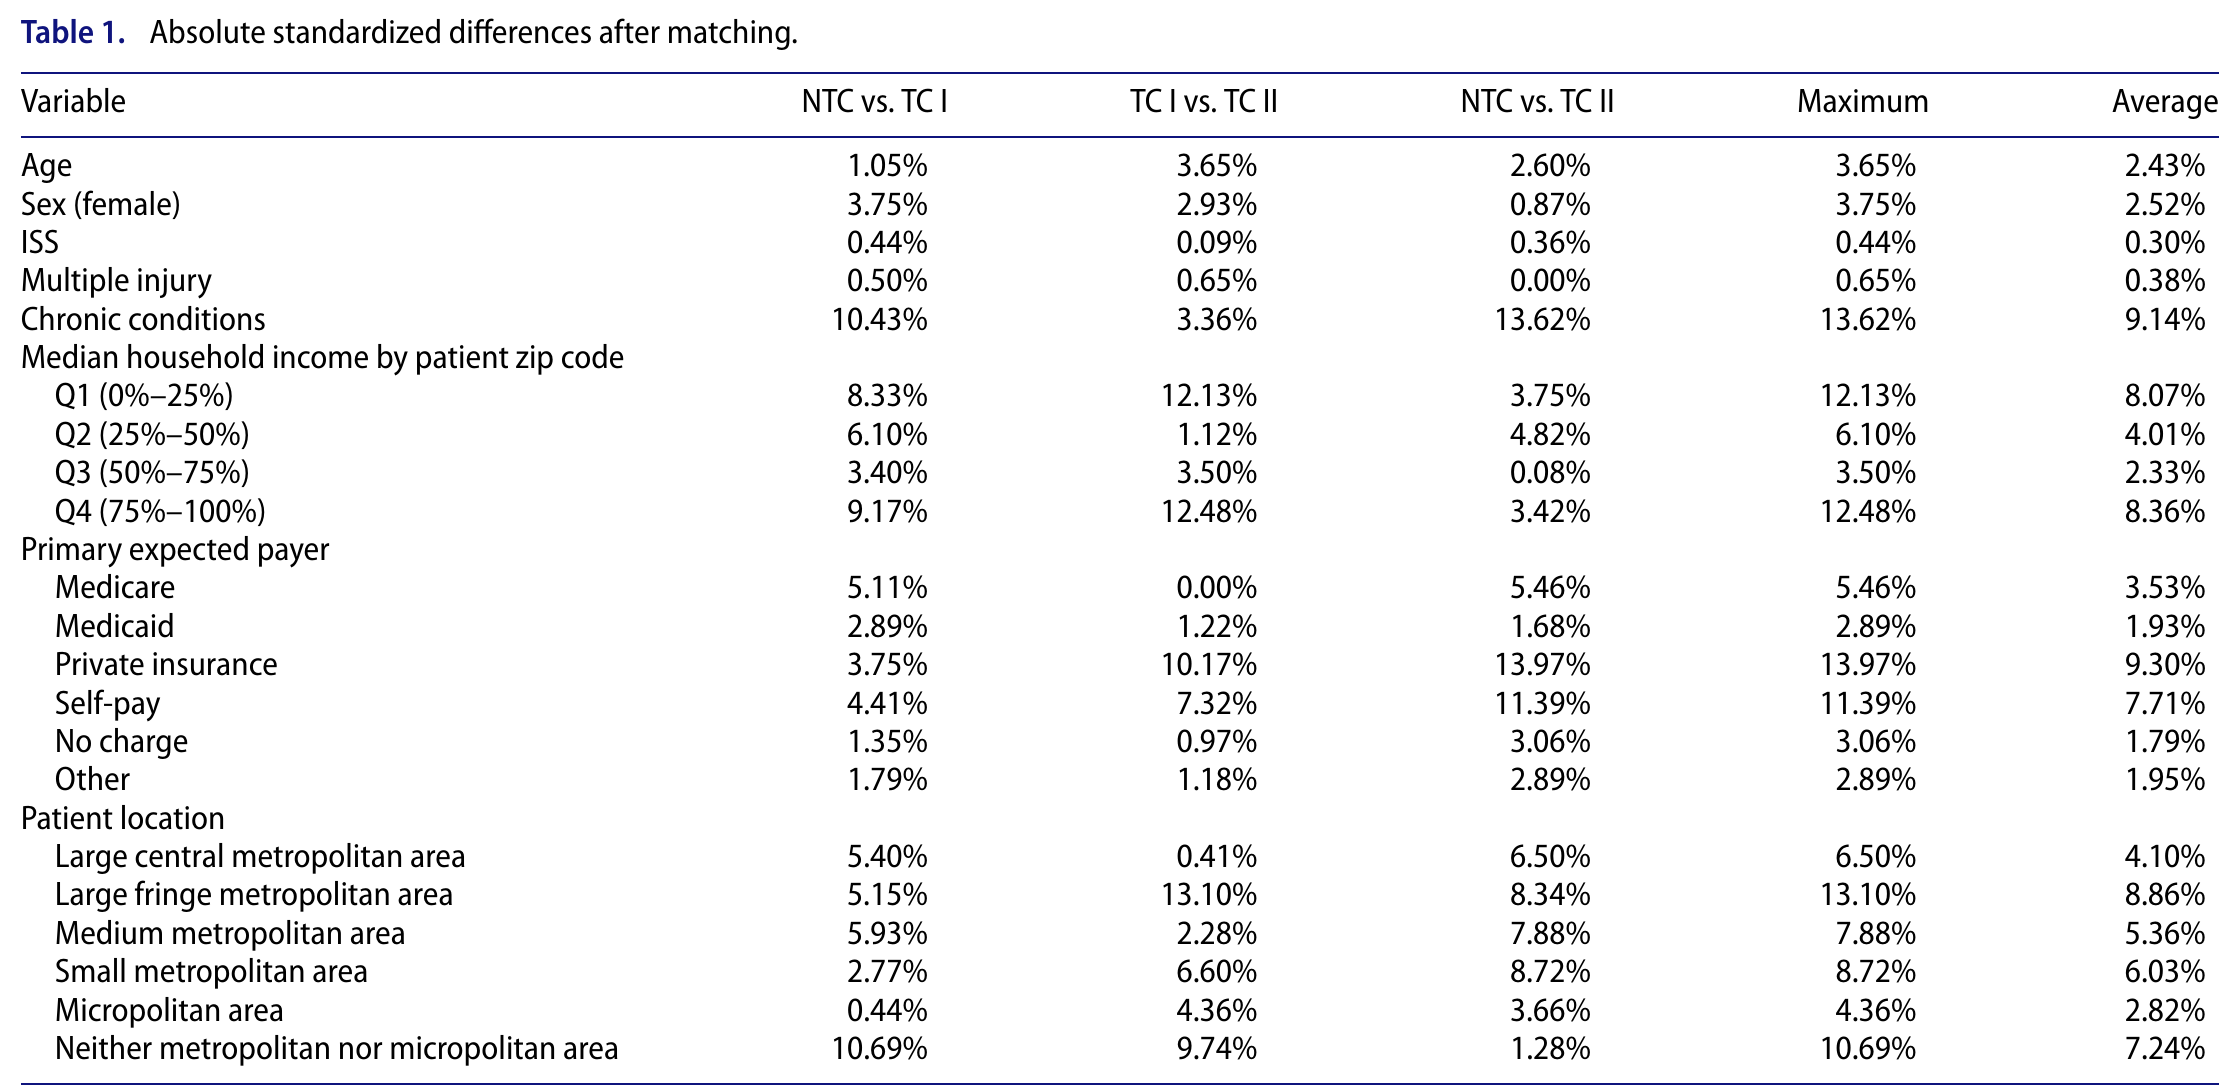
\includegraphics[width=\textwidth]{figures/nattino-table1.png}
    % \caption{\label{fig:label} }
  \end{figure}


  
\end{frame}

% -------------------------------------------------------------------------

\begin{frame}
  \frametitle{Results: Comparisons between trauma centers}

  \begin{figure}[ht]
    \centering
    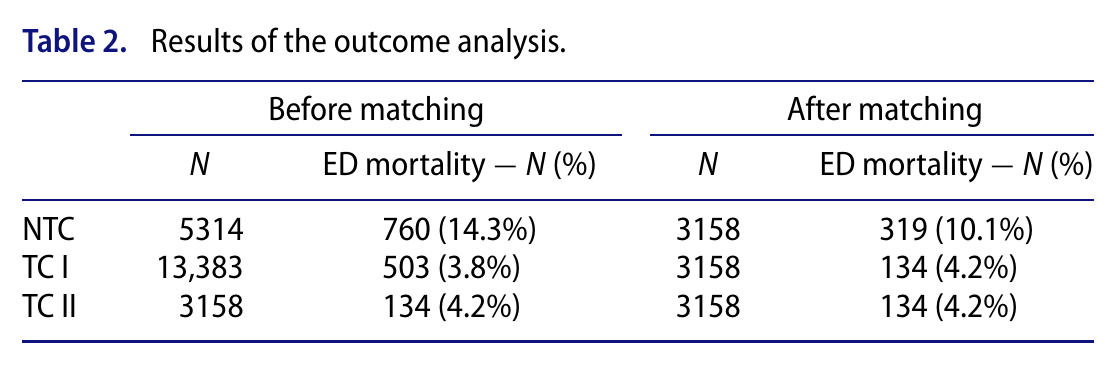
\includegraphics[width=0.7\textwidth]{figures/nattino-table2.png}
    % \caption{\label{fig:label} }
  \end{figure}

  \begin{itemize}
  \item NTC vs TC (TC I and TC II combined): $T_\text{MH}=11.45$, $p<0.001$ \medskip 
  \item TC I vs TC II: $T_\text{MN} = 0$, $p = 0.500$ \medskip 
  \item Assess sensitivity to unobserved confounding
    \citep{rosenbaum1987} gives $\Gamma_{\text{MH}} = 2.34$.
  \end{itemize}
  
\end{frame}

% -------------------------------------------------------------------------

% \begin{frame}
%   \frametitle{Sensiti}
  

  
  
  
% \end{frame}

%%% Local Variables:
%%% mode: latex
%%% TeX-master: "../main"
%%% End:
